\section{Results}
\label{sec:results}

\para{Main-run summary.}
\Tabref{tab:main_summary} gives the aggregate experiment summary. The main run contains 48 model calls, 600 target records, and 536 predicted records. The mean per-run omission rate is 4.17\%, while hallucination and duplicate rates are both 0. The mean field-error rate among matched records is 0.43\%, driven by two action-field errors. All unit, object, count, month, and severity errors are 0 after normalization.

\begin{table}[t]
    \centering
    \begin{tabular}{@{}lr@{}}
        \toprule
        \textbf{Quantity} & \textbf{Value} \\
        \midrule
        Runs & 48 \\
        Target records & 600 \\
        Predicted records & 536 \\
        Parse failures & 2 \\
        Mean per-run omission rate & 4.17\% \\
        Mean per-run hallucination rate & {\bf 0.00\%} \\
        Mean per-run duplicate rate & {\bf 0.00\%} \\
        Mean per-run field-error rate among matched records & 0.43\% \\
        Mean per-run exact-record rate over target records & 95.42\% \\
        \bottomrule
    \end{tabular}
    \caption{Overall main-run results. Rates are means over runs, matching the scoring summary. Hallucination and duplicate rates are best possible and shown in \textbf{bold}.}
    \label{tab:main_summary}
\end{table}


\begin{figure}[t]
    \centering
    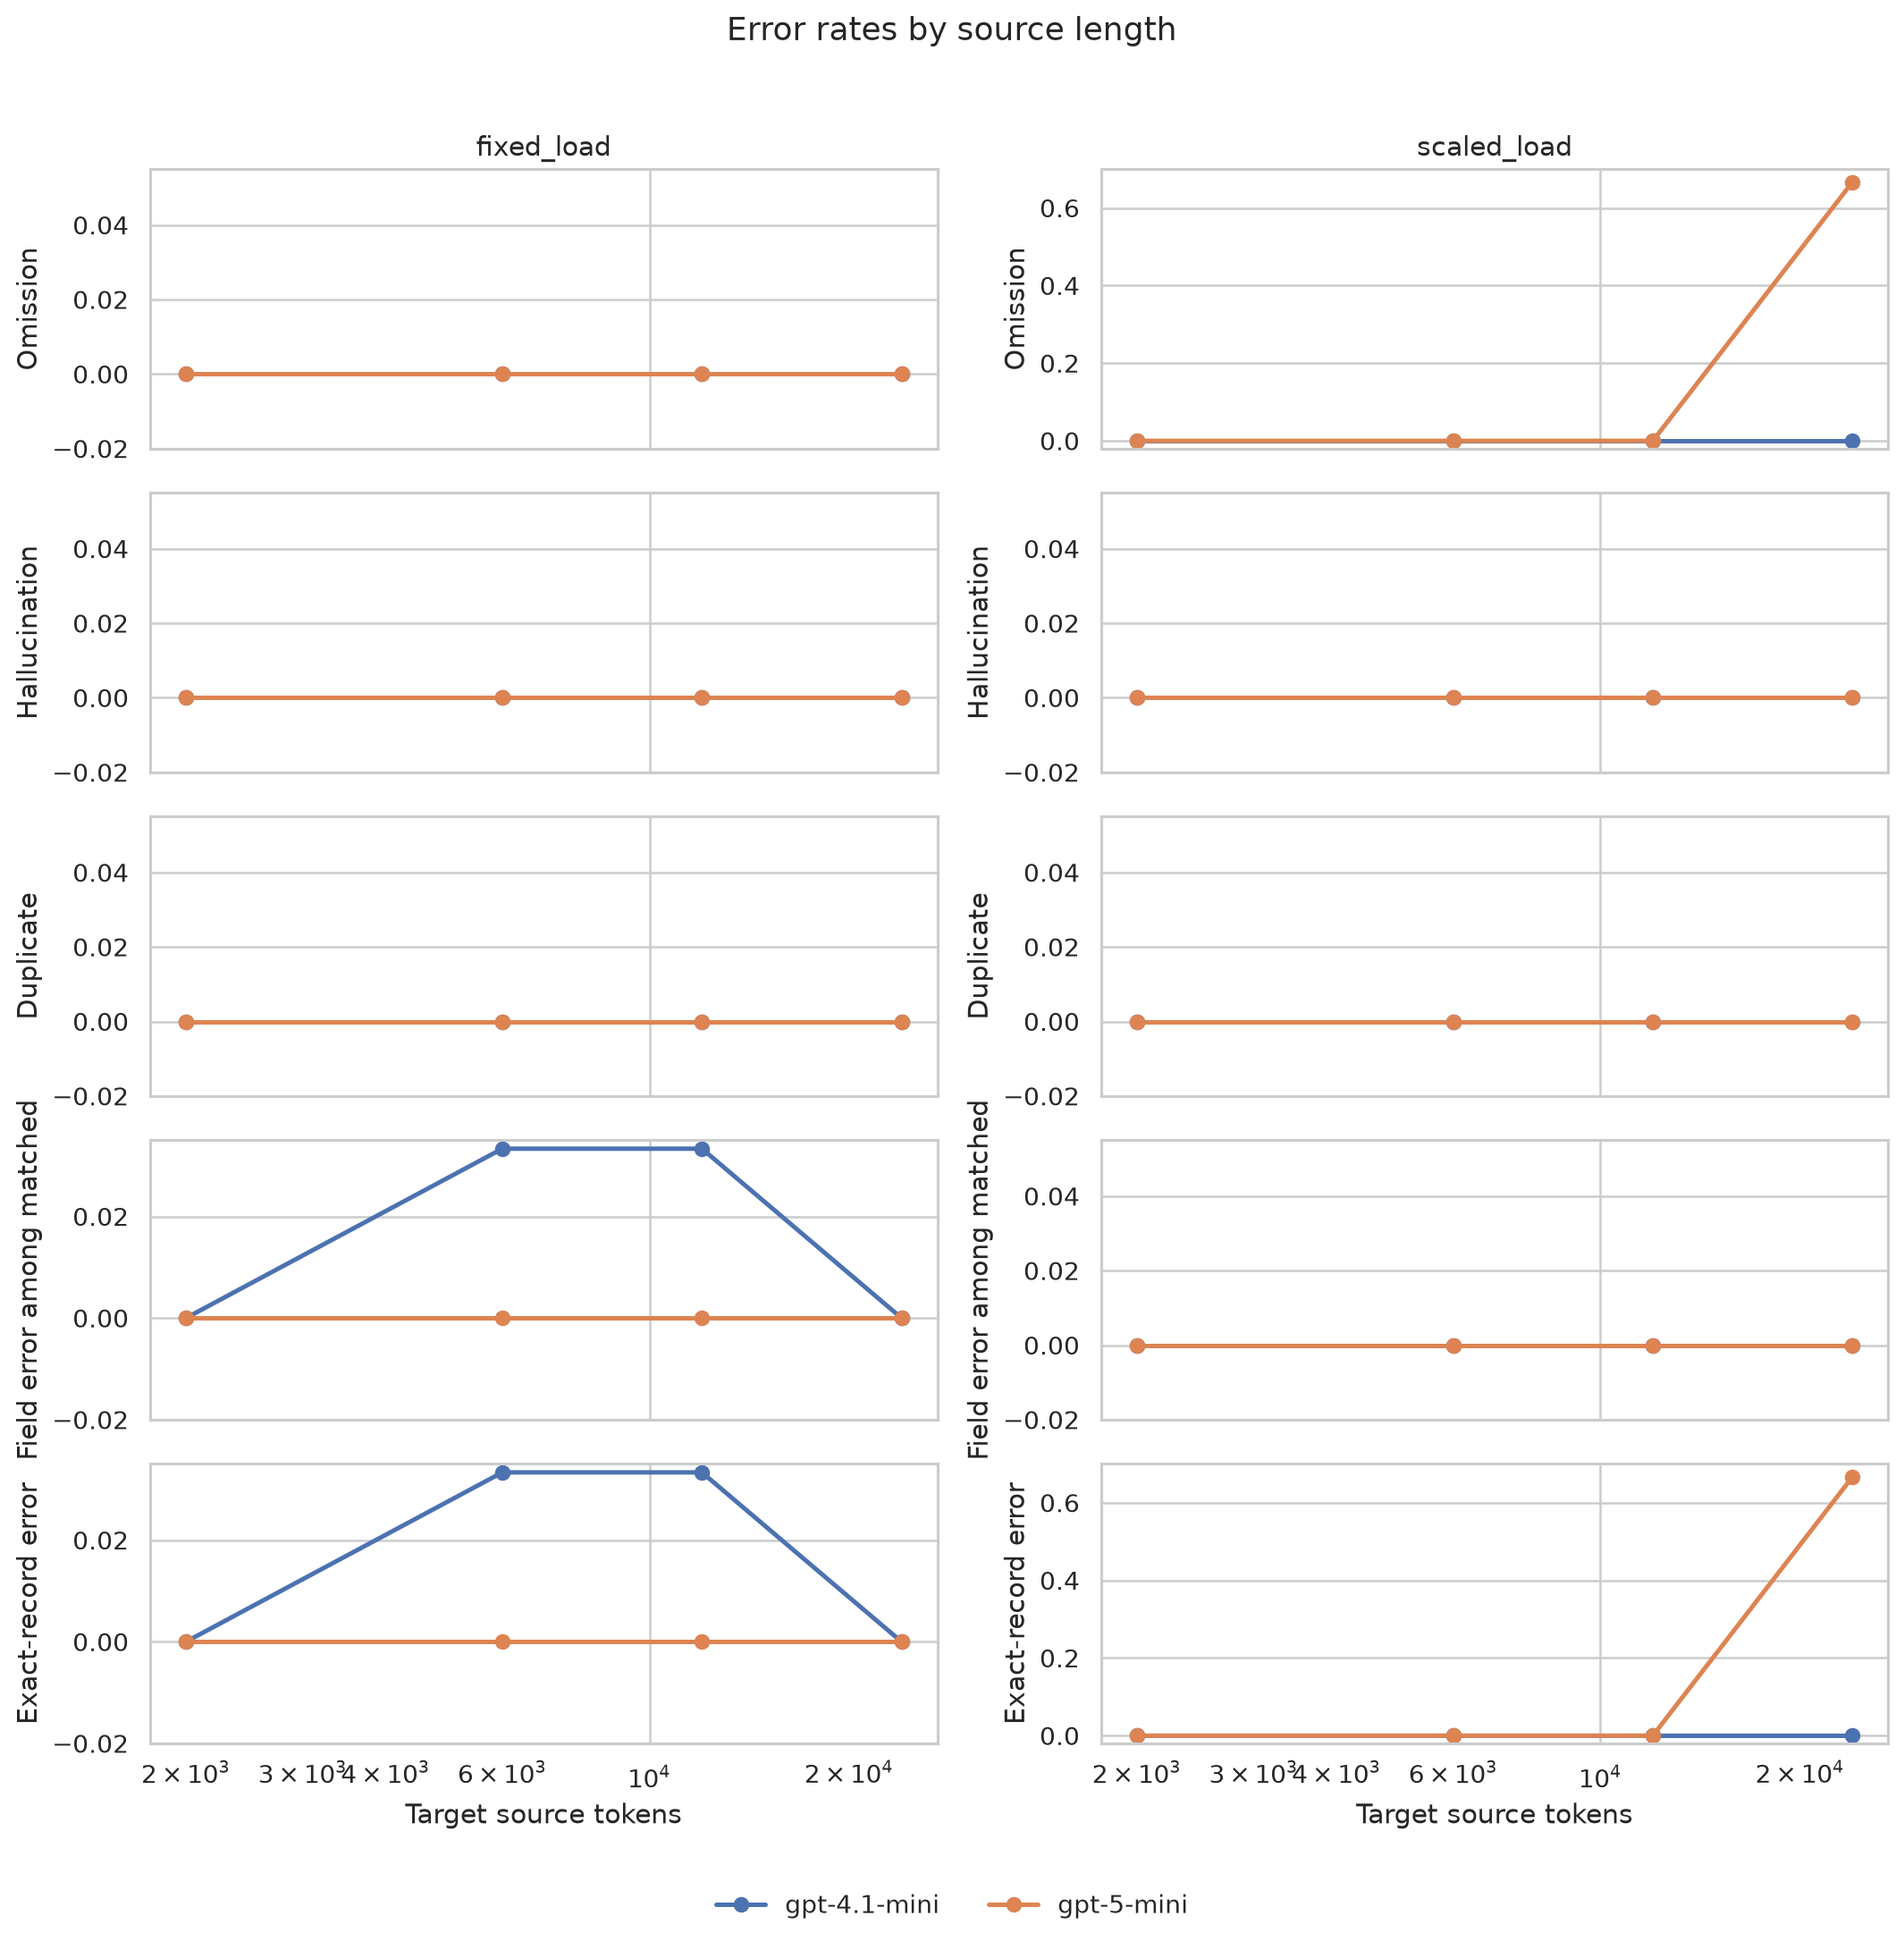
\includegraphics[width=0.86\linewidth]{figures/error_rates_by_length.png}
    \caption{Error rates by source length for each model and task family. Most factual error categories remain at zero across length. The visible increase in omission and exact-record error is concentrated in the \gptfivemini \scaledload 24k-token condition, where two runs return empty visible content under the 5,000-token completion cap.}
    \label{fig:error_rates}
\end{figure}

\para{Valid outputs are nearly exact.}
The mean omission rate falls to 0 when parse failures are excluded. In those 46 valid runs, hallucination and duplicate rates remain 0, and the mean exact-record rate rises to 99.57\%. This means the apparent omission growth in the main run is not caused by partial missed facts inside otherwise valid JSON. It comes from two empty visible outputs in the hardest condition.

\para{The hardest condition separates the models.}
\Tabref{tab:hardest_condition} focuses on the 24k-token bin. \gptfourmini returns all records in both fixed and scaled load, including all 96 records in the 32-fact scaled-load condition. \gptfivemini also returns all records in the 10-fact fixed-load condition. Its only failure is the 32-fact scaled-load condition: two of three runs terminate by length with empty visible content, producing 64 missing records and a mean omission rate of 66.7\%.

\begin{table}[t]
    \centering
    \resizebox{\textwidth}{!}{%
    \begin{tabular}{@{}llcccccc@{}}
        \toprule
        \textbf{Model} & \textbf{Family} & \textbf{Facts} & \textbf{Parse failures} & \textbf{Omission} & \textbf{Hallucination} & \textbf{Duplicate} & \textbf{Exact record} \\
        \midrule
        \gptfourmini & \fixedload & 10 & {\bf 0/3} & {\bf 0.0\%} & {\bf 0.0\%} & {\bf 0.0\%} & {\bf 100.0\%} \\
        \gptfourmini & \scaledload & 32 & {\bf 0/3} & {\bf 0.0\%} & {\bf 0.0\%} & {\bf 0.0\%} & {\bf 100.0\%} \\
        \gptfivemini & \fixedload & 10 & {\bf 0/3} & {\bf 0.0\%} & {\bf 0.0\%} & {\bf 0.0\%} & {\bf 100.0\%} \\
        \gptfivemini & \scaledload & 32 & 2/3 & 66.7\% & {\bf 0.0\%} & {\bf 0.0\%} & 33.3\% \\
        \bottomrule
    \end{tabular}
    }
    \caption{Performance in the 24k-token condition. The only large error rate appears for \gptfivemini under scaled load, where two of three responses contain no visible JSON because the main-run completion budget is exhausted. Best values are in \textbf{bold}.}
    \label{tab:hardest_condition}
\end{table}


\para{A larger completion budget recovers the failures.}
\Tabref{tab:recovery} shows the high-budget recovery check. The two failed \gptfivemini 24k-token, 32-fact tasks recover completely with \texttt{max\_completion\_tokens=12000}. Both runs stop normally, return all 32 records, and have zero hallucinations, duplicates, and field errors. The recovered runs use 2,752 and 2,560 reasoning tokens, respectively, showing that the main-run failures were budget-sensitive rather than evidence-retrieval failures.

\begin{table}[t]
    \centering
    \resizebox{\textwidth}{!}{%
    \begin{tabular}{@{}lcccccc@{}}
        \toprule
        \textbf{Task} & \textbf{Target facts} & \textbf{Parse failure} & \textbf{Missing} & \textbf{Field errors} & \textbf{Reasoning tokens} & \textbf{Completion tokens} \\
        \midrule
        \texttt{scaled\_load-24000-0} & 32 & {\bf 0} & {\bf 0} & {\bf 0} & 2,752 & 4,900 \\
        \texttt{scaled\_load-24000-1} & 32 & {\bf 0} & {\bf 0} & {\bf 0} & 2,560 & 4,706 \\
        \bottomrule
    \end{tabular}
    }
    \caption{High-budget recovery for the two failed \gptfivemini scaled-load 24k runs. Increasing the completion cap from 5,000 to 12,000 tokens recovers every record with zero missing records and zero field errors. Best values are in \textbf{bold}.}
    \label{tab:recovery}
\end{table}


\para{Length slopes reflect separation at one corner case.}
\Tabref{tab:slopes} reports logistic slope tests. Omission grows in the main run under pooled and scaled-load analyses, with Benjamini-Hochberg adjusted $p=0.0040$. Exact-record error also grows in scaled load. However, the odds ratios are infinite because all omission events occur at the largest scaled-load bin. Field errors remain approximately stable: the fixed-load action-error odds ratio is 1.09 per doubling of source tokens with adjusted $p=0.8703$.

\begin{table}[t]
    \centering
    \resizebox{\textwidth}{!}{%
    \begin{tabular}{@{}llccl@{}}
        \toprule
        \textbf{Outcome} & \textbf{Scope} & \textbf{Odds ratio per 2x tokens} & \textbf{BH-adjusted $p$} & \textbf{Interpretation} \\
        \midrule
        Omission & Pooled adjusted & $\infty$ & {\bf 0.0040} & Grows in the main run. \\
        Omission & Scaled load & $\infty$ & {\bf 0.0040} & Grows in the main run. \\
        Exact-record error & Scaled load & $\infty$ & {\bf 0.0040} & Grows in the main run. \\
        Any field error & Fixed load & 1.09 & 0.8703 & Approximately stable. \\
        Action error & Fixed load & 1.09 & 0.8703 & Approximately stable. \\
        \bottomrule
    \end{tabular}
    }
    \caption{Logistic length-slope tests. Infinite odds ratios indicate separation: all omission events occur in the largest scaled-load bin. Significant values are in \textbf{bold}.}
    \label{tab:slopes}
\end{table}


\begin{figure}[t]
    \centering
    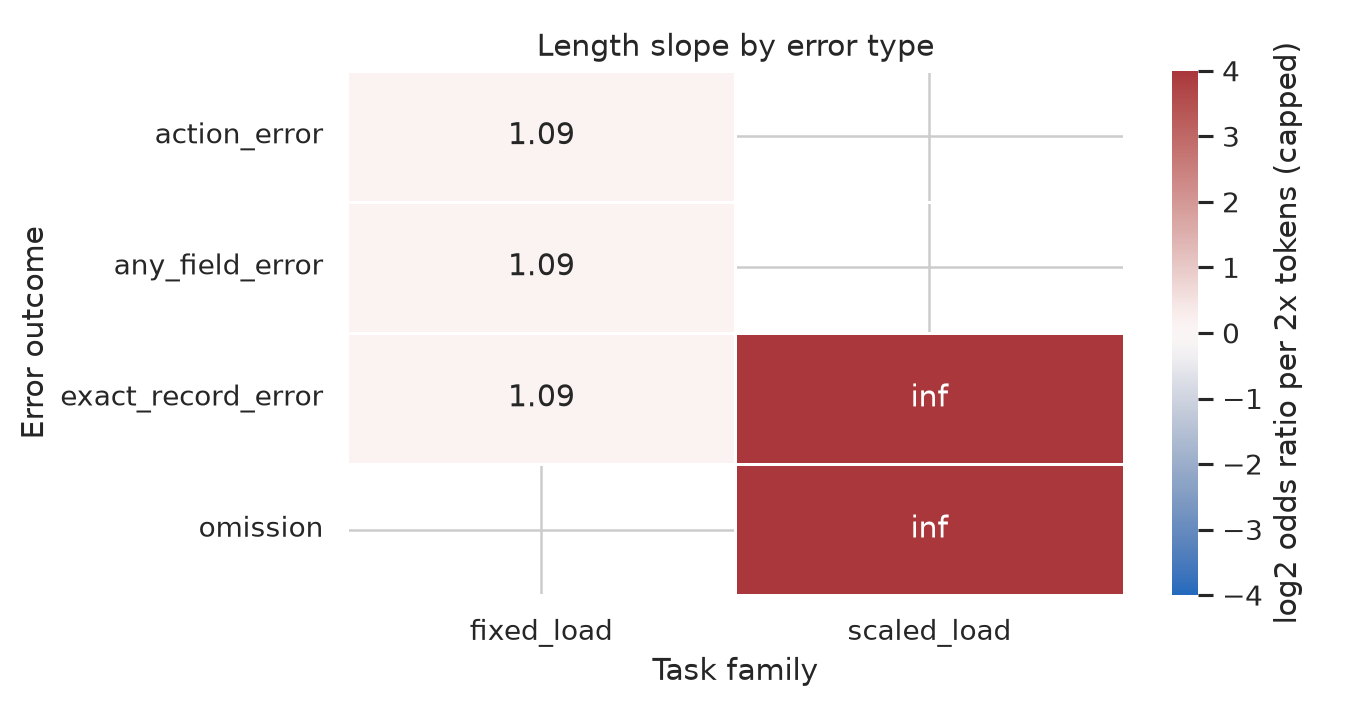
\includegraphics[width=0.95\linewidth]{figures/length_slope_heatmap.png}
    \caption{Length-slope heatmap for tested error indicators. Significant main-run slopes appear for omissions and scaled-load exact-record errors, but these effects are separation artifacts caused by two empty \gptfivemini outputs at the largest scaled-load bin. Field-error slopes are small and statistically indistinguishable from zero.}
    \label{fig:slope_heatmap}
\end{figure}
